% 第 25 题正四棱柱图：按固定源内容流矢量层精确值复刻（1 pt → 0.03515 cm）。
% 原点取顶点 B（源页 (359.64, 566.64) pt），y 向上。
% 实线 9 段（正面/顶面/右侧面可见棱）；虚线 3 条（隐藏竖棱 A–A₁、隐藏底棱 A–D、
% 空间对角线 B–D₁＝题干所指 D₁B），虚线样式照源：节长 2.28、节距 5.22（源为填充短划，此处以 dash 近似）。
% 图不按比例：图上高:底棱 = 72:57 = 1.26，题设解为 1.5——源内示意图，照录不臆改。
% 标签照源为「基线左端」定位（anchor=base west）；八个顶点均无点记号。
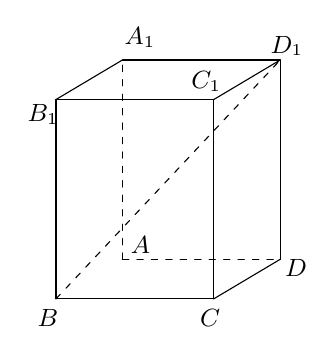
\begin{tikzpicture}[line cap=round,line join=round,font=\small,x=0.03515cm,y=0.03515cm]
% ===== 实线（9 段）=====
\draw (0,0)--(0,72);   % B–B1
\draw (0,0)--(57,0);   % B–C
\draw (57,0)--(57,72);   % C–C1
\draw (0,72)--(57,72);   % B1–C1
\draw (0,72)--(24,86.28);   % B1–A1
\draw (24,86.28)--(81,86.28);   % A1–D1
\draw (81,86.28)--(81,14.28);   % D1–D
\draw (81,14.28)--(57,0);   % D–C
\draw (81,86.28)--(57,72);   % D1–C1
% ===== 虚线（3 条；照源节长/节距）=====
\draw[dash pattern=on 2.28pt off 2.94pt] (24,14.28)--(24,86.28);   % A–A1
\draw[dash pattern=on 2.28pt off 2.94pt] (24,14.28)--(81,14.28);   % A–D
\draw[dash pattern=on 2.28pt off 2.94pt] (0,0)--(81,86.28);   % B–D1
% ===== 标注（照源基线左端，显式坐标）=====
\node[anchor=base west,inner sep=0] at (26.88,16.2) {\(A\)};
\node[anchor=base west,inner sep=0] at (-6.84,-9.96) {\(B\)};
\node[anchor=base west,inner sep=0] at (51.84,-9.96) {\(C\)};
\node[anchor=base west,inner sep=0] at (82.56,8.04) {\(D\)};
\node[anchor=base west,inner sep=0] at (24.6,91.8) {\(A_{1}\)};
\node[anchor=base west,inner sep=0] at (-10.44,64.08) {\(B_{1}\)};
\node[anchor=base west,inner sep=0] at (48.72,75.84) {\(C_{1}\)};
\node[anchor=base west,inner sep=0] at (77.28,88.8) {\(D_{1}\)};
\end{tikzpicture}
